\chapter{Обработка исключений изнутри: условия и перезапуск}
\label{ch:19}

Одной из замечательных особенностей Lisp является его система \textit{условий}. Она служит
тем же целям, что и системы обработки исключений в Java, Python и C++, но является более
гибкой. На самом деле её способности выходят за пределы обработки ошибок~-- условия
являются более всеохватывающими, чем исключения, в том смысле, что условия могут
представить любое событие во время выполнения программы, которое может представлять
интерес в программировании различных уровней стека вызовов. Например, в разделе
<<\nameref{ch19:other-appls}>> вы увидите, что условия могут быть использованы для выдачи
предупреждения без нарушения выполнения кода, который выдаёт предупреждение, в то же время
позволяя коду выше на стеке вызовов контролировать, напечатано ли предупреждающее
сообщение. Пока, однако, я сосредоточусь на обработке ошибок.

Система условий более гибка, чем система исключений, потому что вместо разделения на две
части между кодом, который сигнализирует об ошибке\footnote{Выбрасывает (throw) или
  вызывает (raise) исключение в терминах Java/Python.}, и кодом, который обрабатывает
её\footnote{Ловит (catch) исключение в терминах Java/Python.}, система условий разделяет
ответственность на три части~-- \textit{сигнализация} условия, его \textit{обработка} и
\textit{перезапуск}. В этой главе я опишу, как можно использовать условия в гипотетическом
приложении для анализа журнальных файлов. Вы увидите, как можно использовать систему
условий, чтобы дать возможность низкоуровневой функции обнаружить проблему в процессе
разбора журнального файла и сигнализировать об ошибке, коду на промежуточном уровне
предоставить несколько возможных путей исправления такой ошибки и коду на высшем уровне
приложения определить политику для выбора стратегии исправления.

Для начала я введу некоторую терминологию: \textit{ошибки}, как я буду использовать этот
термин, есть последствие закона Мёрфи. Если может случиться что-то плохое, оно случится:
файл, который ваша программа должна прочесть, будет потерян, диск, на который вам надо
записать, будет полон, сервер, с которым вы общаетесь, упадёт, или исчезнет сеть. Если
что-то из этих вещей случилось, это может помешать участку кода выполнить то, что вы
хотите. Но это не программная ошибка: нет места в коде, которое вы можете исправить, чтобы
сделать несуществующий файл существующим или освободить место на диске. Однако если
оставшаяся часть программы зависит от действий, которые должны были быть сделаны, то вам
лучше как-то разобраться с происшествием, иначе вы ошибку \textit{закладываете}. Итак,
ошибки не всегда бывают программными, но их игнорирование~-- это всегда ошибка в
программе.

Что же означает обработать ошибку? В хорошо написанной программе каждая функция~-- это
чёрный ящик, скрывающий внутреннее содержание своей работы. Программы, таким образом,
строятся из функций разных уровней: функции на высшем уровне построены на функциях более
низкого уровня и~т.д.  Эта иерархия функционирования выражается во время выполнения в
форме стека вызовов: когда \emph{высший} вызывает \emph{среднего}, а он, в свою очередь,
вызывает \emph{нижнего}, то поток выполнения находится внизу, но он также проходит через
\emph{средний} и \emph{высший} уровни, поэтому они все находятся в одном стеке вызовов.

Так как каждая функция является чёрным ящиком, связи между функциями~-- прекрасное место
для работы с ошибками. Каждая функция~-- \emph{нижняя} для примера~-- должна делать
какую-то работу. Та, которая её непосредственно вызывает,~-- \emph{средняя} в нашем случае
~-- рассчитывает на неё в своей работе. Однако ошибка, которая мешает ей сделать свою
работу, подвергает всех вызывающих риску: \emph{средняя} вызывала \emph{нижнюю}, потому
что ей нужна работа, которую \emph{нижняя} делает; если эта работа не сделана, у
\emph{средней} проблемы. Но это означает, что у вызвавшей \emph{среднюю}, \emph{высшей},
тоже проблемы~-- и так далее вверх по стеку вызовов вплоть до верха программы. С другой
стороны, так как каждая функция~-- чёрный ящик, если какая-то функция в стеке вызовов может
как-то сделать свою работу, несмотря на проблемы у тех, кто пониже, то никакой функции
повыше не надо знать, что проблемы вообще были,~-- все эти функции заботятся, только чтобы
функции, которых они вызывают, как-то сделали работу, которую от них ждут.

В большинстве языков ошибки обрабатываются путём возврата из упавшей функции и передачи
шанса вызывающей функции или всё исправить, или упасть самой. Некоторые языки используют
обычный механизм возврата из функций, в то время как языки с исключениями возвращают
контроль через \textit{выброс} или \textit{возбуждение} исключения. Исключения~-- это
огромное усовершенствование над использованием обычных возвратов функций, но обе схемы
страдают от общего порока: пока ищется функция, которая может восстановиться, стек
пустеет. Это приводит к тому, что код, который может всё восстановить, должен сделать это
без контекста того, что код нижнего уровня пытался сделать, когда случилась ошибка.

Рассмотрим гипотетическую цепочку вызовов из \emph{высшей}, \emph{средней}, \emph{нижней}
функций. Если \emph{нижняя} падает и \emph{средняя} не может всё поправить, дело
передаётся в суд высшей инстанции. Для \emph{высшей}, чтобы обработать ошибку, надо или
сделать свою работу без помощи \emph{средней}, или как-то всё изменить, чтобы вызов
\emph{средней} работал, и вызвать её снова. Первый вариант теоретически прост, но
предполагает кучу лишнего кода~-- полное воплощение того, что, предполагалось, сделает
\emph{средняя}. И чем дальше стек освобождается, тем больше работы, которую следует
переделать. Второй вариант~-- исправление ситуации и ещё одна попытка~-- запутанный:
для \emph{высшей}, чтобы иметь возможность изменить ситуацию в мире так, чтобы второй
вызов \emph{средней} не закончился ошибкой в \emph{нижней}, необходимо неподобающее ей
знание внутреннего устройства обеих функций: \emph{средней} и \emph{нижней}, что
противоречит идее, что каждая функция является чёрным ящиком.

\section{Путь языка Lisp}

Система обработки ошибок в языке Common Lisp даёт вам выход из этого тупика, позволяя вам
отделить код, который исправляет ошибки, от кода, который решает, как их исправлять. Таким
образом, вы можете поместить код восстановления в функции низкого уровня, на самом деле не
обязывая использовать какую-то конкретную стратегию восстановления, предоставляя решать
это коду функций высшего уровня.

Чтобы почувствовать, как это работает, предположим, что вы пишете приложение, которое
читает какой-то текстовый файл наподобие журнала веб-сервера. Где-то в вашем приложении
будет ваша функция разбора отдельных журнальных записей. Давайте предположим, что вы
напишете функцию \lstinline{parse-log-entry}, которой будет передаваться строка, содержащая
одну журнальную запись, и которая предположительно вернёт объект \lstinline{log-entry},
представляющий эту запись. Эта функция будет вызываться из функции \lstinline{parse-log-file},
которая читает журнальный файл полностью и возвращает список объектов, представляющий все
записи в журнале.

Чтобы всё упростить, от функции \lstinline{parse-log-entry} не будет требоваться разбирать
неправильно сформированные записи. Однако она будет способна распознать, когда её ввод
неправилен. Но что она должна делать, когда она определяет неправильный ввод? В языке C вы
бы вернули специальное значение, чтобы обозначить, что была проблема. В~языках Java или
Python вы бы выбросили или возбудили исключение. В~Common Lisp вы сигнализируете условие.

\section{Условия}

\textit{Условие}~-- это объект, чей класс обозначает общую природу условия, а данные
экземпляров класса несут информацию о деталях конкретных обстоятельств, которые приводят к
сигнализации об условии\footnote{В этом аспекте условия очень похожи на исключения в Java
  или Python, разве что не все условия представляют ошибку или исключительную ситуацию.}. В
нашей гипотетической программе анализа журнальных файлов вы можете определить класс
условия \lstinline{malformed-log-entry-error}, с помощью которого \lstinline{parse-log-entry} будет
сигнализировать, если предоставленные ему данные он не сможет разобрать.

Классы условий определяются макросом \lstinline{DEFINE-CONDITION}, который работает точно так
же, как \lstinline{DEFCLASS}, исключая то, что суперклассом по умолчанию для классов,
определённых с \lstinline{DEFINE-CONDITION}, является \lstinline{CONDITION}, а не
\lstinline{STANDARD-OBJECT}. Слоты определяются так же, и классы условий могут иметь
единственное или множественное наследование от других классов, которые происходят от
\lstinline{CONDITION}. Однако, по историческим причинам от классов условий не требуется быть
экземплярами \lstinline{STANDARD-OBJECT}, так что некоторые из функций, которые вы используете
и классы которых созданы через \lstinline{DEFCLASS}, не обязательно должны работать с
условиями. В частности, слоты условий недоступны для \lstinline{SLOT-VALUE}: вы должны задать
или опцию \lstinline{:reader}, или опцию \lstinline{:accessor} для любого слота, чьё значение вы
собираетесь использовать. Точно так же новые объекты для условий создаются путём вызова
\lstinline{MAKE-CONDITION}, а не \lstinline{MAKE-INSTANCE}. \lstinline{MAKE-CONDITION} инициализирует
слоты нового условия, основываясь на полученных \lstinline{:initarg}, но способа последующей
настройки инициализации условия, аналогичного \lstinline{INITIALIZE-INSTANCE}, не
существует\footnote{В некоторых реализациях языка Common Lisp условия определены как
  подкласс от \lstinline{STANDARD-OBJECT}, в этом случае \lstinline{SLOT-VALUE},
  \lstinline{MAKE-INSTANCE} и \lstinline{INITIALIZE-INSTANCE} будут работать, но на это нельзя
  полагаться из-за непереносимости.}.

При использовании системы условий для обработки ошибок вы должны определять ваши условия
как подклассы \lstinline{ERROR}, который является, в свою очередь, подклассом
\lstinline{CONDITION}. Таким образом, вы можете определить условие
\lstinline{malformed-log-entry-error} со слотом для хранения аргумента, который был передан в
\lstinline{parse-log-entry}, вот так:

\begin{myverb}
(define-condition malformed-log-entry-error (error)
  ((text :initarg :text :reader text)))
\end{myverb}

\section{Обработчики условий}

В \lstinline{parse-log-entry} вы будете сигнализировать \lstinline{malformed-log-entry-error}, если
вы не сможете разобрать журнальную запись. Вы сигнализируете об ошибках функцией
\lstinline{ERROR}, которая вызывает низкоуровневую функцию \lstinline{SIGNAL} и попадает в отладчик,
если условие не обрабатывается. Можно вызвать \lstinline{ERROR} двумя путями: послать ей уже
сформированный объект условия или послать ей имя класса условия и любые аргументы
инициализации, необходимые для построения нового условия, и она создаст его для вас.
Первое иногда полезно для повторной сигнализации уже существующего объекта условия, а
второе более лаконично. Итак, вы можете записать \lstinline{parse-log-entry} в таком виде,
опуская детали собственно разбора журнальной записи:

\begin{myverb}
(defun parse-log-entry (text)
  (if (well-formed-log-entry-p text)
    (make-instance 'log-entry ...)
    (error 'malformed-log-entry-error :text text)))
\end{myverb}

То, что происходит, когда сигнализируется ошибка, зависит от кода в стеке вызовов,
стоящего выше \lstinline{parse-log-entry}. Чтобы избежать попадания в отладчик, вы должны
установить \textit{обработчик условия} в одну из функций, предшествующих вызову
\lstinline{parse-log-entry}. Когда условие сигнализируется, механизм сигнализирования
просматривает список активных обработчиков условий, ищя по классу условия обработчик,
способный обработать сигнализируемое условие. Каждый обработчик условия состоит из
спецификатора типа, обозначающего, какие типы условий он может обработать, и функции,
которая получает единственный аргумент~-- условие. В каждый момент времени может быть
несколько активных обработчиков этого условия на различных уровнях стека вызовов. Когда
условие сигнализируется, механизм сигнализирования находит последний установленный
обработчик, чей спецификатор типа совместим с сигнализируемым условием и вызывает его
функцию, передавая ей объект условия.

Функция обработки может выбрать, обрабатывать ли ей условие. Функция может отказаться
обрабатывать условие, просто нормально завершившись, в этом случае управление возвращается
функции \lstinline{SIGNAL}, которая будет искать следующий установленный обработчик с
подходящим спецификатором типа. Для обработки условия функция обязана передать управление,
минуя функцию \lstinline{SIGNAL} посредством \textit{нелокального выхода}. В следующей секции
вы увидите, как обработчик может выбрать, куда передать контроль. Однако многие
обработчики условий просто хотят опустошить стек до того места, где они были установлены,
и затем запустить некоторый код. Макрос \lstinline{HANDLER-CASE} как раз устанавливает такой
тип обработчика. Базовая форма \lstinline{HANDLER-CASE} такова:

\begin{myverb}
(handler-case expression
  error-clause*)
\end{myverb}

\noindent{}где каждая конструкция \textit{error-clause} представляет собой следующую форму:

\begin{myverb}
(condition-type ([var]) code)
\end{myverb}

Если выражение \textit{expression} завершается нормально, тогда его значение возвращается
из конструкции \lstinline{HANDLER-CASE}. Тело \lstinline{HANDLER-CASE} должно быть одним выражением,
но вы можете использовать \lstinline{PROGN} для объединения нескольких выражений в одну
форму. Если всё же выражение сигнализирует условие, которое является одним из типов
\textit{condition-type}, указанных в одной из секций \textit{error-clause}, то код из
соответствующей секции будет выполнен, и его значение будет возвращено из
\lstinline{HANDLER-CASE}. Если указана переменная \textit{var}, она будет именем переменной,
содержащей объект условия при выполнении кода обработчика. Если код не нуждается в доступе
к объекту условия, вы можете опустить имя переменной.

Например, одним из способов обработки условия \lstinline{malformed-log-entry-error},
сигнализируемого из функции \lstinline{parse-log-entry} в вызывающую её функцию
\lstinline{parse-log-file}, был бы пропуск неправильной записи. В следующей функции выражение
\lstinline{HANDLER-CASE} вернёт либо имя, возвращаемое \lstinline{parse-log-entry}, либо \lstinline{NIL},
если \lstinline{malformed-log-entry-error} сигнализируется. Слово \lstinline{it} во фразе
\lstinline{collect it} цикла \lstinline{LOOP} является ещё одним ключевым словом \lstinline{LOOP},
которое ссылается на значение последнего выполненного условия, в данном случае~-- на
переменную \lstinline{entry}).

\begin{myverb}
(defun parse-log-file (file)
  (with-open-file (in file :direction :input)
    (loop for text = (read-line in nil nil) while text
       for entry = (handler-case (parse-log-entry text)
                     (malformed-log-entry-error () nil))
       when entry collect it)))
\end{myverb}

Когда функция \lstinline{parse-log-entry} завершается нормально, её значение присваивается
переменной \lstinline{entry} и затем накапливается циклом \lstinline{LOOP}. Но если функция
\lstinline{parse-log-entry} сигнализирует ошибку \lstinline{malformed-log-entry-error}, то
обработчик ошибки вернёт \lstinline{NIL}, который не будет сохранён.

%% TODO
%% START OF TABLE
 Обработка исключений в стиле языка Java 

\lstinline{HANDLER-CASE} в языке Common Lisp является ближайшим аналогом стиля обработки
исключений в языках Java и Python. То, что вы можете записать на языке Java как 

\begin{myverb}[language=Java]
try {
  doStuff();
  doMoreStuff();
} catch (SomeException se) {
  recover(se);
}
\end{myverb} 

\noindent{}или на языке Python как 

\begin{myverb}[language=Python]
try:
  doStuff()
  doMoreStuff()
except SomeException, se:
  recover(se)
\end{myverb} 

\noindent{}в языке Common Lisp вы пишете так: 

\begin{myverb}
(handler-case
    (progn
      (do-stuff)
      (do-more-stuff))
  (some-exception (se) (recover se)))
\end{myverb} 

%% END OF TABLE

Эта версия \lstinline{parse-log-file} имеет один серьёзный недостаток: она делает слишком много
всего. Как предполагает её имя, работа \lstinline{parse-log-file} заключается в разборе файла и
выдаче списка объектов \lstinline{log-entry}; если это невозможно, не её дело~-- решать, что
сделать взамен. Что, если вы захотите использовать \lstinline{parse-log-file} в приложении,
которое захочет сказать пользователю, что журнальный файл повреждён, или в таком, которое
захочет восстановить неправильную запись путём исправления её и разбора снова? Или
приложению достаточно пропускать их до тех пор, пока не накопится определённое количество
повреждённых записей.

Вы можете попытаться решить проблему, переместив \lstinline{HANDLER-CASE} в функцию высшего
уровня. Однако тогда у вас не будет способа воплотить текущую политику пропуска отдельных
записей~-- когда ошибка будет просигнализированна, стек будет опустошён вплоть до функции
высшего уровня, разбор журнального файла будет вообще покинут. Что вам надо, так это
способ предоставить текущую стратегию восстановления без требования всегда её
использовать.

\section{Перезапуск}

Система условий позволяет вам это делать через разделение кода обработки ошибок на две
части. Вы помещаете код, который, собственно, исправляет ошибки, в перезапуски (restarts), и
обработчик условия может затем обработать условие, запустив подходящий вариант. Код
перезапуска можно положить в средне- или низкоуровневую функцию, такую как
\lstinline{parse-log-file} или \lstinline{parse-log-entry}, переместив обработчик условия на высший
уровень в приложении.

Для изменения \lstinline{parse-log-file}, чтобы она устанавливала перезапуск вместо обработчика
условия, вы можете сменить \lstinline{HANDLER-CASE} на \lstinline{RESTART-CASE}. Форма
\lstinline{RESTART-CASE} довольно похожа на \lstinline{HANDLER-CASE}, за исключением того, что имена
перезапусков,~-- это просто имена, не обязательно имена типов условия. В общем, имя
перезапуска должно описывать действие, которое перезапуск совершает. В
\lstinline{parse-log-file} вы можете вызвать перезапуск \lstinline{skip-log-entry}, так как он делает
именно <<пропустить журнальную запись>>. Новая версия будет выглядеть так:

\begin{myverb}
(defun parse-log-file (file)
  (with-open-file (in file :direction :input)
    (loop for text = (read-line in nil nil) while text
       for entry = (restart-case (parse-log-entry text)
                     (skip-log-entry () nil))
       when entry collect it)))
\end{myverb}

Если вы вызовете эту версию \lstinline{parse-log-file} на журнальном файле, содержащем
повреждённую запись, она не обработает ошибку напрямую; вы попадёте в отладчик. Однако
там среди различных представленных перезапусков от отладчика будет один, называемый
\lstinline{skip-log-entry}, который, если вызовете его, продолжит выполнение
\lstinline{parse-log-file} дальше в прежнем режиме. Для избежания попадания в отладчик вы
можете установить обработчик условия, который вызовет перезапуск \lstinline{skip-log-entry}
автоматически.

Преимущество установки перезапуска вместо обработки ошибки напрямую в
\lstinline{parse-log-file} в том, что это даёт возможность использовать \lstinline{parse-log-file} в
большем количестве ситуаций. Код высшего уровня, который вызывает \lstinline{parse-log-file},
не обязан вызывать перезапуск \lstinline{skip-log-entry}. Он может выбрать обработку ошибки на
высшем уровне. Или, как я покажу в следующей секции, вы можете добавить перезапуск в
\lstinline{parse-log-entry}, чтобы предоставить другую стратегию исправления, и затем обработчик
условия может выбрать, какую стратегию он хочет использовать.

Но перед этим вам надо увидеть, как установить обработчик условия, который будет вызывать
\lstinline{skip-log-entry} перезапуск. Вы можете установить обработчик где угодно в
цепочке вызовов, ведущей к \lstinline{parse-log-file}. Это может быть довольно высокий
уровень в вашем приложении, не обязательно в функции, непосредственно вызывающей
\lstinline{parse-log-file}. Например, предположим, что главная точка входа в ваше
приложение~-- это функция \lstinline{log-analyzer}, которая ищет стопку журналов и
анализирует их функцией \lstinline{analyze-log}, которая в итоге приводит к вызову
\lstinline{parse-log-file}. Без какой-либо обработки ошибок это может выглядеть так:

\begin{myverb}
(defun log-analyzer ()
  (dolist (log (find-all-logs))
    (analyze-log log)))
\end{myverb}

Работа \lstinline{analyze-log}~-- это вызвать прямо или непрямо \lstinline{parse-log-file} и затем
сделать что-то с возвращённым списком журнальных записей. Сверхпростая версия может
выглядеть так:

\begin{myverb}
(defun analyze-log (log)
  (dolist (entry (parse-log-file log))
    (analyze-entry entry)))
\end{myverb}

\noindent{}где функция \lstinline{analyze-entry} предположительно ответственна за извлечение заботящей вас
информации про каждую журнальную запись и припрятывание её куда-нибудь.

Таким образом, путь от функции высшего уровня \lstinline{log-analyzer} к
\lstinline{parse-log-entry}, которая, собственно, сигнализирует про ошибку, следующий:

\begin{figure}[h]
  \centering
  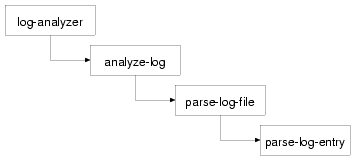
\includegraphics[scale=0.7]{images/restart-call-stack.png}
\end{figure}

Предполагая, что вы всегда хотите пропускать неправильно сформированные записи, вы можете
изменить эту функцию для установки обработчика условия, который вызывает перезапуск
\lstinline{skip-log-entry} для вас. Однако вы не можете использовать \lstinline{HANDLER-CASE} для
установки обработчика условия, потому что тогда стек будет опустошён до функции, где
\lstinline{HANDLER-CASE} появляется. Вместо этого вам надо использовать макрос нижнего уровня
\lstinline{HANDLER-BIND}. Основная форма \lstinline{HANDLER-BIND} следующая:

\begin{myverb}
(handler-bind (binding*) form*)
\end{myverb}

\noindent{}где каждая привязка (binding) представляет собой список из типа условия и
обрабатывающей функции с одним аргументом. После провязок с обработчиками тело
\lstinline{HANDLER-BIND} может содержать произвольное число форм. В отличие от кода
обработчика в \lstinline{HANDLER-CASE}, код обработчика должен быть функцией и должен
принимать единственный аргумент. Более важным различием между \lstinline{HANDLER-BIND} и
\lstinline{HANDLER-CASE} является то, что функция обработки, привязанная через
\lstinline{HANDLER-BIND}, будет запущена без опустошения стека~-- поток контроля будет всё
ещё в вызове \lstinline{parse-log-entry}, если эта функция вызвана. Вызов
\lstinline{INVOKE-RESTART} найдёт и вызовет последний связанный перезапуск с данным
именем. Таким образом вы можете добавить обработчик к \lstinline{log-analyzer}, который
будет вызывать \lstinline{skip-log-entry} перезапуск, установленный в
\lstinline{parse-log-file}, таким образом\footnote{Компилятор может возмутиться, если
  параметр нигде не используется. Вы можете подавить это предупреждение, добавив
  объявление \lstinline{(declare (ignore c))} как первое выражение в тело
\lstinline{LAMBDA}.}:

\begin{myverb}
(defun log-analyzer ()
  (handler-bind ((malformed-log-entry-error
                  #'(lambda (c)
                      (invoke-restart 'skip-log-entry))))
    (dolist (log (find-all-logs))
      (analyze-log log))))
\end{myverb}

В этом \lstinline{HANDLER-BIND} обработчик является безымянной функцией, которая вызывает
перезапуск \lstinline{skip-log-entry}. Вы также могли бы определить функцию с именем, которая
делала бы то же самое, и связать всё с ней. Фактически это обычная практика, когда
определение перезапуска является определением функции с тем же именем и, получающей
единственный аргумент, условие, которая вызывает одноимённый перезапуск. Такие функции
называются функциями перезапуска. Можно определить функцию перезапуска
\lstinline{skip-log-entry} так:

\begin{myverb}
(defun skip-log-entry (c)
  (invoke-restart 'skip-log-entry))
\end{myverb}

Затем вы могли бы изменить определение \lstinline{log-analyzer} на такое:

\begin{myverb}
(defun log-analyzer ()
  (handler-bind ((malformed-log-entry-error #'skip-log-entry))
    (dolist (log (find-all-logs))
      (analyze-log log))))
\end{myverb}

Как уже было сказано, функция перезапуска \lstinline{skip-log-entry} полагает, что перезапуск
\lstinline{skip-log-entry} уже был установлен. Если \lstinline{malformed-log-entry-error}
просигнализирован кодом, вызванным из \lstinline{log-analyzer} без уже установленного
\lstinline{skip-log-entry}, вызов \lstinline{INVOKE-RESTART} будет сигнализировать
\lstinline{CONTROL-ERROR}, когда не сможет обнаружить перезапуск \lstinline{skip-log-entry}. Если вы
хотите допустить возможность того, чтобы \lstinline{malformed-log-entry-error} могло быть
просигнализировано из кода, в котором перезапуск \lstinline{skip-log-entry} не установлен, то вы
можете изменить функцию \lstinline{skip-log-entry} таким образом:

\begin{myverb}
(defun skip-log-entry (c)
  (let ((restart (find-restart 'skip-log-entry)))
    (when restart (invoke-restart restart))))
\end{myverb}

\lstinline{FIND-RESTART} ищет перезапуск с данным именем и возвращает объект, представляющий
перезапуск, если перезапуск найден, или \lstinline{NIL}, если нет. Вы можете вызвать перезапуск
путём посылки перезапуск-объекта к \lstinline{INVOKE-RESTART}. Таким образом, когда
\lstinline{skip-log-entry} привязывается внутри \lstinline{HANDLER-BIND}, она будет обрабатывать
условие путём вызова перезапуска \lstinline{skip-log-entry}, если тот доступен, или, в противном
случае, нормально завершится, давая другим обработчикам условия, привязанным выше по
стеку, шанс таки обработать условие.

\section{Предоставление множественных перезапусков}

Так как перезапуски должны быть прямо вызваны, чтобы был какой-то эффект, вы можете
определить несколько перезапусков, предоставляющих различную стратегию исправления. Как я
упоминал ранее, не все приложения для разбора журналов будут обязательно хотеть пропускать
неправильные записи. Некоторые приложения могут захотеть, чтобы \lstinline{parse-log-file}
включала специальный тип объекта для представления неправильной записи в списке
\lstinline{log-entry} объектов; другие приложения могут иметь несколько путей для
восстановления неправильной записи и могут хотеть иметь способ отправки исправленной
записи назад в \lstinline{parse-log-entry}.

Чтобы позволить существовать более сложным протоколам исправления, перезапуски могут
получать произвольные аргументы, которые передаются в вызове \lstinline{INVOKE-RESTART}. Вы
можете предоставить поддержку для обеих стратегий исправления, которые я упомянул, путём
добавления двух перезапусков к \lstinline{parse-log-entry}, каждый из которых получает
единственный аргумент. Первый просто возвращает значение, которое получил, как значение
всего \lstinline{parse-log-entry}, в то время как другой пытается разобрать свой аргумент на
месте оригинальной журнальной записи.

\begin{myverb}
(defun parse-log-entry (text)
  (if (well-formed-log-entry-p text)
    (make-instance 'log-entry ...)
    (restart-case (error 'malformed-log-entry-error :text text)
      (use-value (value) value)
      (reparse-entry (fixed-text) (parse-log-entry fixed-text)))))
\end{myverb}

Имя \lstinline{USE-VALUE} является стандартным именем для такого типа перезапуска. Common Lisp
определяет функцию для \lstinline{USE-VALUE} аналогично \lstinline{skip-log-entry} функции, только
что вами определённой. Таким образом, если вы хотели изменить политику по отношению к
неправильным записям на ту, которая создана экземпляром \lstinline{malformed-log-entry}, вы
могли бы сменить \lstinline{log-analyzer} на такую функцию (предполагая существование
\lstinline{malformed-log-entry} класса с инициирующим аргументом \lstinline{:text}):

\begin{myverb}
(defun log-analyzer ()
  (handler-bind ((malformed-log-entry-error
                  #'(lambda (c)
                      (use-value
                       (make-instance 'malformed-log-entry :text (text c))))))
    (dolist (log (find-all-logs))
      (analyze-log log))))
\end{myverb}

Вы могли бы точно так же поместить эти новые перезапуски в \lstinline{parse-log-file} вместо
\lstinline{parse-log-entry}. Хотя вы, вообще-то, хотите поместить перезапуски в код
по возможности самого нижнего уровня. Не было бы, однако, правильным перемещать перезапуск
\lstinline{skip-log-entry} в \lstinline{parse-log-entry}, так как это может привести к возвращению
иногда \lstinline{'NIL} от \lstinline{parse-log-entry} в качестве результата нормального завершения,
а вы начинали всё с тем, чтобы таких вещей избежать. И это была бы одинаково плохая идея~--
убрать перезапуск \lstinline{skip-log-entry}, исходя из теории, что обработчик условия смог бы
достичь того же эффекта через вызов-перезапуск \lstinline{use-value} с \lstinline{NIL} в качестве
аргумента; это потребовало бы от обработчика условия знания внутренней работы
\lstinline{parse-log-file}. Таким образом, \lstinline{skip-log-entry}~-- правильно абстрагированная
часть API журнального разбора.

\section{Другие применения условий}
\label{ch19:other-appls}

В то время как условия в основном используются для обработки ошибок, они также могут быть
использованы для других целей~-- вы можете применить условия, обработчики условий и
перезапуски для конструирования различных протоколов между низко- и высокоуровневым
кодом. Ключом для понимания возможностей условий является понимание того, что просто
сигнализация условия не влияет на поток контроля.

Примитивная сигнальная функция \lstinline{SIGNAL} воплощает механизм поиска применимого
обработчика условия и вызывает его обрабатывающую функцию. Причина, почему обработчик
может отказаться обрабатывать условие и нормально завершиться,~-- потому что вызов
функции обработчика,~-- это обычный вызов функции: когда обработчик завершается, контроль
передаётся обратно к \lstinline{SIGNAL}, которая затем ищет другой, ранее привязанный
обработчик, который может обработать условие. Если \lstinline{SIGNAL} исчерпает обработчики
условия до того, как условие будет обработано, она также завершается нормально.

Ранее использованная вами функция \lstinline{ERROR} вызывает \lstinline{SIGNAL}. Если ошибка
обрабатывается обработчиком условия, который передаёт управление через \lstinline{HANDLER-CASE}
или через вызов перезапуска, тогда вызов \lstinline{SIGNAL} никогда не завершится. Но если
\lstinline{SIGNAL} завершается, \lstinline{ERROR} вызывает отладчик путём вызова функции,
сохранённой в \lstinline{*DEBUGGER-HOOK*}. Таким образом, вызов \lstinline{ERROR} никогда не сможет
завершиться нормально; условие должно быть обработано или обработчиком условия, или в
отладчике.

Другая сигнализирующая условие функция \lstinline{WARN} представляет пример протокола ещё
одного типа, построенный на системе условий. Подобно \lstinline{ERROR}, \lstinline{WARN}
вызывает \lstinline{SIGNAL} для сигнализации условия. Но если \lstinline{SIGNAL}
завершается, \lstinline{WARN} не вызывает отладчик~-- она печатает условие в
\lstinline{*ERROR-OUTPUT*} и возвращает \lstinline{NIL}, позволяя своему вызывающему
продолжать работу. \lstinline{WARN} также устанавливает перезапуск
\lstinline{MUFFLE-WARNING}, обёртку вокруг вызова \lstinline{SIGNAL}, которая может быть
использована обработчиком условия, чтобы сделать возврат из \lstinline{WARN} без печатания
чего-либо. Функция \lstinline{MUFFLE-WARNING} перезапуска ищет и вызывает одноимённый
перезапуск, сигнализируя \lstinline{CONTROL-ERROR}, если такого перезапуска нет. Конечно,
условие, сигнализируемое \lstinline{WARN}, также может быть обработано другим путём~--
обработчик условия может <<\textit{поспособствовать}>>, чтобы предупреждение об ошибке
обрабатывалось, как если бы ошибка действительно была.

Например, в приложении для разбора журналов, если журнальная запись немного неправильна, но
всё же поддаётся разбору, вы могли бы указать \lstinline{parse-log-entry} разобрать немного
повреждённую запись, но сигнализировать \lstinline{WARN}, когда она будет делать это. Затем
большее приложение может выбрать либо позволить предупреждению быть напечатанным, либо
скрыть предупреждение, либо рассматривать предупреждение как ошибку, исправляя ситуацию,
как это делалось при \lstinline{malformed-log-entry-error}.

Третья сигнализирующая ошибки функция, \lstinline{CERROR}, представляет ещё один протокол.
Подобно \lstinline{ERROR}, \lstinline{CERROR} сбросит вас в отладчик, если условие, которая она
сигнализирует, не будет обработано. Однако, как и \lstinline{WARN}, она устанавливает перезапуск
перед сигнализацией условия. Перезапуск, \lstinline{CONTINUE}, приведёт к нормальному
завершению \lstinline{CERROR}~-- если перезапуск был вызван обработчиком условия, он вообще
сохранит вас от попадания в отладчик. В противном случае вы можете использовать
перезапуск, как только окажетесь в отладчике для продолжения вычислений сразу после вызова
\lstinline{CERROR}. Функция \lstinline{CONTINUE} находит и вызывает \lstinline{CONTINUE} перезапуск, если
он доступен, и возвращает \lstinline{NIL} в противном случае.

Вы также можете конструировать ваши собственные протоколы поверх \lstinline{SIGNAL}~-- везде,
где низкоуровневый код нуждается в передаче информации назад по стеку вызовов в
высокоуровневый код, механизм условий является подходящим механизмом для использования. Но
для большинства целей один из стандартных протоколов ошибок или предупреждений должен
подойти.

Вы будете использовать систему условий в будущих практических главах как в виде обычной
обработки ошибок, так и, в \ref{ch:25}-й главе, для помощи в обработке мудрёного особого случая при
разборе ID3-файлов.  К сожалению, это судьба обработки ошибок, всегда идти мелким шрифтом
в программных текстах~-- надлежащая обработка ошибок или отсутствие таковой является
часто наибольшим отличием иллюстративного кода и утяжелённого кода промышленного качества.
Хитрость написания последнего относится больше к принятию особого строгого образа мышления
о программном обеспечении, чем к деталями конструкции языка. Так что если вашей целью
является написание такого типа программ, то вы найдёте систему условий в Common Lisp
отличным инструментом для написания надёжного кода и прекрасно подходящей для стиля
последовательных улучшений (incremental development style).

%% TODO
%% START OF TABLE
Написание надёжных программ 

Для информации по написанию надёжных программ нет ничего лучше, чем начать с поиска книги
Гленфорда Мейерса <<Надёжность программного обеспечания>> (\textit{Software Reliability},
Glenford J. Meyers, John Wiley \& Sons, 1976).  Написанное Бертрандом Мейером (Bertrand
Meyer) про <<контрактное программирование>> (Design By Contract) также показывает полезный
путь в размышлениях про правильность программ.  Например, смотрите главы~11 и~12 его книги
\textit{Object-Oriented Software Construction} (Prentice Hall, 1997). Запомните, однако,
что Бертранд Мейер является изобретателем Eiffel, статически типизированного
крепостнического и дисциплинарного языка из школы Algol/Ada. Хотя у него есть много умных
мыслей про объектную ориентированность и программную надёжность, всё же существует
довольно большой разрыв между его видением программирования и путём Lisp. Наконец, для
прекрасного обзора большинства проблем, окружающих построение отказоустойчивых систем,
смотрите главу 3 из классической \textit{Transaction Processing: Concepts and Techniques}
(Morgan Kaufmann, 1993) от Джима Грея (Jim Gray) и Андреаса Ройтера (Andreas Reuter).

%% END OF TABLE

В следующей главе я дам быстрый обзор некоторых из 25 специальных операторов, которых у
вас пока не было шанса использовать, по крайней мере прямо.

%%% Local Variables: 
%%% mode: latex
%%% TeX-master: "pcl-ru"
%%% TeX-open-quote: "<<"
%%% TeX-close-quote: ">>"
%%% End: 
